%%%%%%%%%%%%%%%%%%%%%%%%%%%%%%%%%%%%%%%%%
% Thin Sectioned Essay
% LaTeX Template
% Version 1.0 (3/8/13)
%
% This template has been downloaded from:
% http://www.LaTeXTemplates.com
%
% Original Author:
% Nicolas Diaz (nsdiaz@uc.cl) with extensive modifications by:
% Vel (vel@latextemplates.com)
%
% License:
% CC BY-NC-SA 3.0 (http://creativecommons.org/licenses/by-nc-sa/3.0/)
%
%%%%%%%%%%%%%%%%%%%%%%%%%%%%%%%%%%%%%%%%%

%----------------------------------------------------------------------------------------
%	PACKAGES AND OTHER DOCUMENT CONFIGURATIONS
%----------------------------------------------------------------------------------------

\documentclass[a4paper, 11pt]{article} % Font size (can be 10pt, 11pt or 12pt) and paper size (remove a4paper for US letter paper)

\usepackage[protrusion=true,expansion=true]{microtype} % Better typography
\usepackage{graphicx} % Required for including pictures
\usepackage{wrapfig} % Allows in-line images

\usepackage{mathpazo} % Use the Palatino font
\usepackage[T1]{fontenc} % Required for accented characters
\linespread{1.05} % Change line spacing here, Palatino benefits from a slight increase by default

\usepackage[utf8]{inputenc}
\usepackage[colorlinks, pdfpagelabels, pdfstartview = FitH, bookmarksopen = true, bookmarksnumbered = true, linkcolor = black, plainpages = false, hypertexnames = false, citecolor = black] {hyperref}
\usepackage{hyphenat}

\makeatletter
\renewcommand\@biblabel[1]{\textbf{#1.}} % Change the square brackets for each bibliography item from '[1]' to '1.'
\renewcommand{\@listI}{\itemsep=0pt} % Reduce the space between items in the itemize and enumerate environments and the bibliography

\renewcommand{\maketitle}{ % Customize the title - do not edit title and author name here, see the TITLE block below
\begin{flushright} % Right align
{\LARGE\@title} % Increase the font size of the title

\vspace{50pt} % Some vertical space between the title and author name

{\large\@author} % Author name
\\\@date % Date

\vspace{40pt} % Some vertical space between the author block and abstract
\end{flushright}
}

%----------------------------------------------------------------------------------------
%	TITLE
%----------------------------------------------------------------------------------------

\title{\textbf{Dokumentation des Medida Projekts "Uniknigge"}\\ % Title
von Hung Tran Duc, Elizaveta Ragosina, Philipp Plotz, Christoph Jurkowski, Niklas Fallik und Sheyda Hayatgheybi} % Subtitle

\author{\textsc{Gruppe 1 (Tutorin: Bianca Preißler)} % Author
\\{\textit{Technische Universität Dresden}}} % Institution

\date{16.07.2015} % Date

%----------------------------------------------------------------------------------------

\begin{document}

\maketitle % Print the title section

%----------------------------------------------------------------------------------------
%	ABSTRACT AND KEYWORDS
%----------------------------------------------------------------------------------------

\renewcommand{\abstractname}{Präambel} % Uncomment to change the name of the abstract to something else

\vspace{5cm} % Some vertical space between the abstract and first section


\begin{abstract}
\noindent
Die hier vorliegende Dokumentation des Mediendidaktik und -psychologie Praktikums der Gruppe 1 mit Hung Tran Duc, Elizaveta Ragosina, Philipp Plotz, Christoph Jurkowski, Niklas Fallik und Sheyda Hayatgheybi legt die Vorstellung des Spiels, Technische Umsetzung, Evaluation mit der Zielgruppe, Projektverlauf
und eigenes Fazit sowie ein Statement von jedem Gruppenmitglied dar. Das Lernspiel "Uniknigge" basiert auf dem weitverbreiteten Adobe Flash und bildet zusammen mit allerhand Mini-Spielen und Grafiken ein vollständiges Spiel.
\end{abstract}

% \hspace*{3,6mm}\textit{Keywords:} lorem , ipsum , dolor , sit amet , lectus % Keywords

\newpage 
\section*{Historie}
Wichtige Änderungen und zugehörige ausführende Autoren.\\
\begin{tabular}{|lllp{5.5cm}|}
\hline 
\textbf{Version} & \textbf{Datum} & \textbf{Autor(en)} & \textbf{Bemerkungen} \\ 
\hline 
0.1 & 16.07.2015 & Christoph Jurkowski & \nohyphens{Erstellung der Struktur, Präambel, Einfügen von Dokumentationsteilen} \\ 
\hline
\end{tabular} 


%----------------------------------------------------------------------------------------
%	ESSAY BODY
%----------------------------------------------------------------------------------------

\newpage
\renewcommand{\contentsname}{Inhaltsverzeichnis}
\tableofcontents

\newpage
\section{Einführung}
Diese Dokumentation beschäftigt sich mit der Umsetzung des Lernspiels "Uniknigge" von der Idee bis zum vollständigen Spiel durch die Entwickler und Grafiker Hung Tran Duc, Elizaveta Ragosina, Philipp Plotz, Christoph Jurkowski, Niklas Fallik und Sheyda Hayatgheybi.

\section{Vorstellung des Spiels}
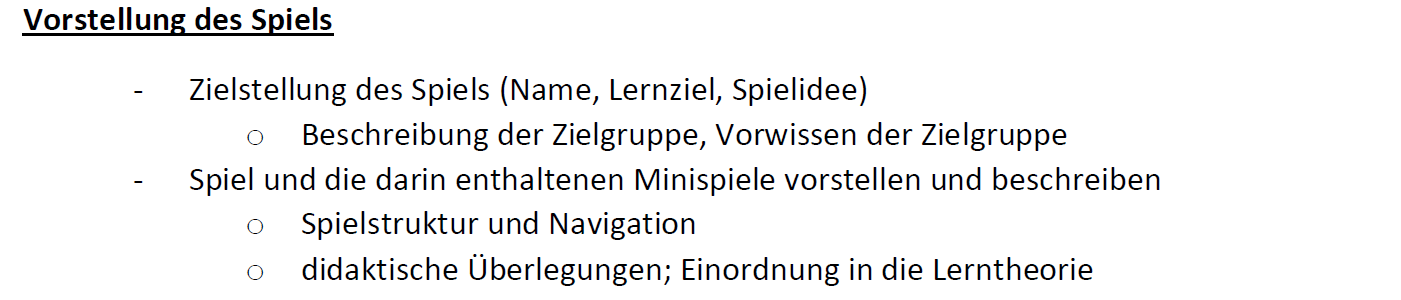
\includegraphics[scale=0.5]{images/vorstellung.png}\\\\
Unsere Grundidee war es ein Lernspiel zu entwickeln, welches als universalen Verhaltenskodex für angehende Studenten, am Beispiel eines Informatikstudenten der TU Dresden, dient. An den Verhaltenskodex angelehnt haben wir unser Spiel „Uniknigge“ genannt. Unsere Zielgruppe sind angehende Studenten, die kurz vor dem Antritt ihres Erststudiums sind, also praktisch zwischen der Immatrikulation und dem ersten Tag in der Universität. Dabei benötigt der Spieler keinerlei spezifische Vorkenntnisse, sondern soll intuitiv nach bestem Gewissen agieren. \\

Das Spiel selbst führt den Spieler durch einen fiktiven ersten Tag in der Uni und stellt ihn immer wieder vor soziale wie auch intellektuelle Herausforderungen. Die Herausforderungen werden in der Spielstory wie auch in den Minispielen offensichtlich oder versteckt gestellt. Während des Intros wird dem Spieler in Form einer Smartphone App eine ausführliche Erklärung, welche man jederzeit im Spiel wieder aufrufen kann, zur Verfügung gestellt. Zusätzlich werden vor jedem Minispiel, weitere Regeln zum Verhalten wie auch zur Spielanwendung bereitgestellt. Nach den Minispielen, wie auch bei Herausforderungen während des Spiels, wird eine kurze Auswertung gezeigt mit eventuellem Lob. Am Ende des Spiels folgt eine längere Resolution mit Verweisen auf jeweilige Herausforderungen mit Verbesserungsvorschlägen für den nächsten Spielablauf. Da unser Spiel eine Verhaltensanleitung darstellt, ist das Ziel und die Zielfindung erst mal nicht klar erkennbar und wird erst während des Spiels sichtbar.
Das Ziel ist es eine Balance, zwischen dem aufmerksamen, leistungsfokussierten Lernen und den Studiums überlebenswichtigen Sozialkompetenzen, zu erreichten.

\section{Technische Umsetzung}
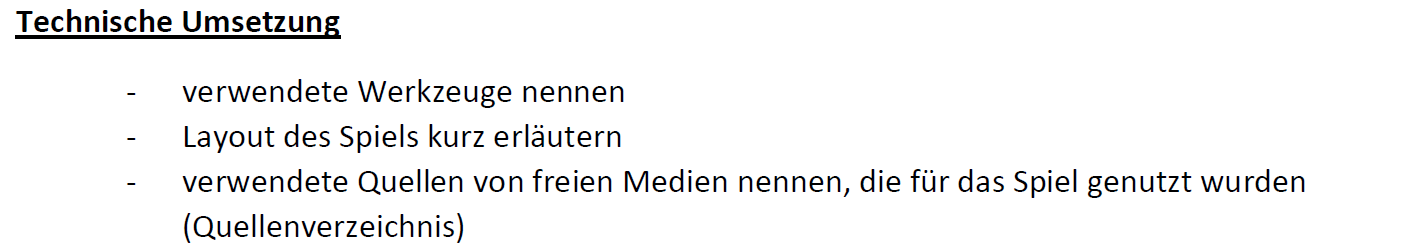
\includegraphics[scale=0.5]{images/umsetzung.png}\\\\
\subsection{Layout}
\subsection{Allgemeines}
\subsection{Hauptmenü}
Unser Hauptmenü, wie auch alle weiteren Spielsequenzen haben als Hintergrund ein Foto, das in Photoshop bearbeitet, einen Comic ähnlichen Eindruck erweckt. Diesen Stil haben wir auch auf die Figuren und weiteren Gegenstände übertragen.
Zusätzlich ist im Hauptmenü der Schriftzug „Uniknigge“ und drei Buttons vorhanden. Die Buttons sind zum Spiel starten, Spiel fortsetzen und zur aktuellen Punkteabfrage. Das Hauptmenü dient der Einstimmung des Spielers auf das Spiel und die Spielumgebung.

\subsection{Intro}
Wie bereits erwähnt, zieht sich unser Layout aus Comic ähnlichen Bildern durch das ganze Spiel. Das Intro ist eine kleine Filmsequenz, der den Spieler in die Problematik und Aufgabenstellung, wie auch Anwendungen beispielsweise das Handy, einführt. Zu sehen ist ein Student, der vor seinem ersten Unitag nicht schlafen kann und um ihm die Angst zunehmen, bekommt er einen Handy App mit Regeln, Anweisungen und Tipps.

\subsection{Spielablauf}
Der Spielablauf ist als "Point-and-Click“ Anwendung konzipiert. Entscheidungen der häufig durch einen Mitspieler eingeleitet in Form von Sprechblasen.
Auch die Punkte Übersicht und der zeitlich Fortschritt des gesamten Spiels sind zu jeder Zeit sichtbar in Form von Balken beziehungsweise einer Uhr.

\subsection{Minispiele}
Vom Design, sind die Minispiele im bewohnten Comic Layout gehalten, doch in Gegensatz zu dem herkömmlichen Spielablauf, werden hierfür die Pfeiltasten zur Bedienung herangezogen. Das hat den Effekt, dass der Spieler merkt, das bei diesen Aufgaben mehr von ihm verlangt wird, als im Spielablauf. Zum dem kann er auch die Maus benutzen, um die Anwendung zu pausieren.

\subsection{Das Smartphone}
Das Handy dient als Informationslieferant, jederzeit im Spiel bietet es dem Spieler die Möglichkeit Fakten und Verhaltensregeln in allgemeinen oder auch zur spezifischen Situation nachzulesen.
Die Informationen sind passend, zu der immerwährenden Abrufung in einer Handy App.

\subsection{Outro}
Das Outro ist an das Intro angelehnt, der Student befindet sich nach seinem ersten Tag wieder in seinem Bett, dort denkt der über den Tag nach. Er bekommt über seine Handy App die Evaluation mit Tipps und Anmerkungen zu seinen Entscheidungen. 

\subsection{Hilfsmittel}



\section{Evaluation mit der Zielgruppe}
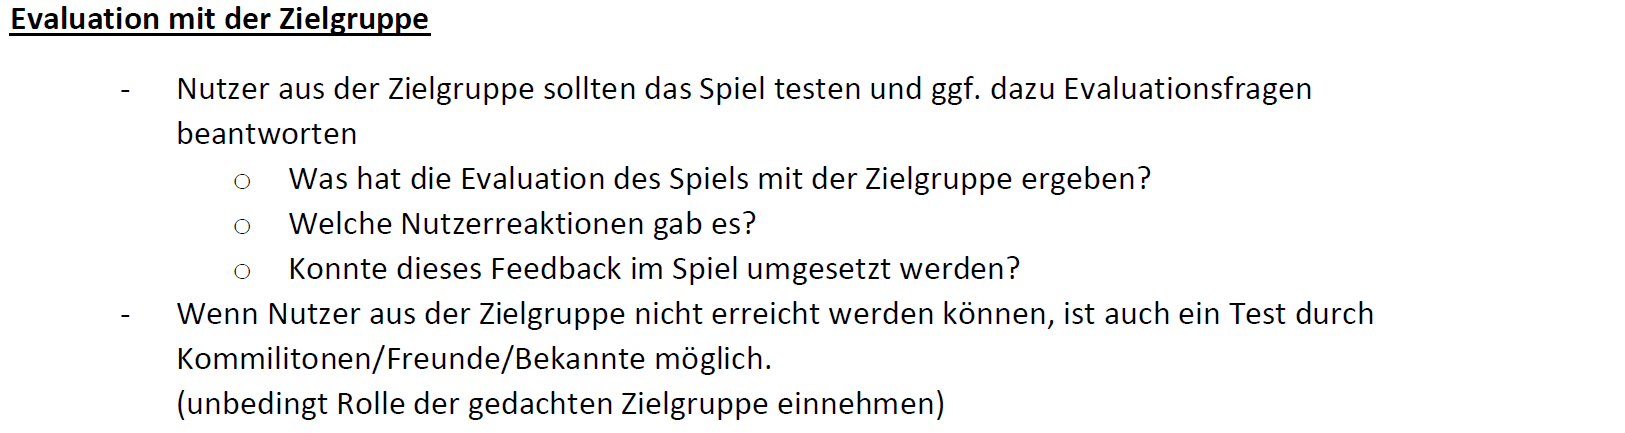
\includegraphics[scale=0.5]{images/evaluation.png}\\\\
Das Lernspiel gibt angehenden Studenten, die zwischen der Immatrikulierung und der ersten Vorlesungszeit stehen die Möglichkeit den Unialltag spielerisch in seiner Vielseitigkeit kennenzulernen. Ausgerichtet auf diesen Anspruch haben wir die Bedienungen, Texte und Aufgaben auf einem hohen Niveau, damit sie die angehenden Studenten damit identifizieren können. Neben dem spielerischen Aspekt kann das Lernspiel auch auf den Webseiten von Universitäten und Berufsorientierungsportalen zu Verfügung gestellt werden. Abiturienten können durch das Spiel Fragen wie zum Beispiel "Wie sieht der Unialltag aus?“, "Wie finde ich mich an der Uni zurecht?“ oder "Wie komme ich in Kontakt mit anderen Studenten?“ klären. Um Spielatmosphäre während des Spielens und Lernen etwas aufzulockern, Haben fiktive Elemente, wie Karlchen, welcher dem Spieler Nachts die Smartphone App empfiehlt, eingebaut. Zudem sind die Minispiele überzogene Anlehnungen an unsere eigenen Erfahrungen an das erste Semester. Ein Beispiel das jeder Student kennt ist das Labyrinth zur Raumfindung. 
\section{Projektverlauf}
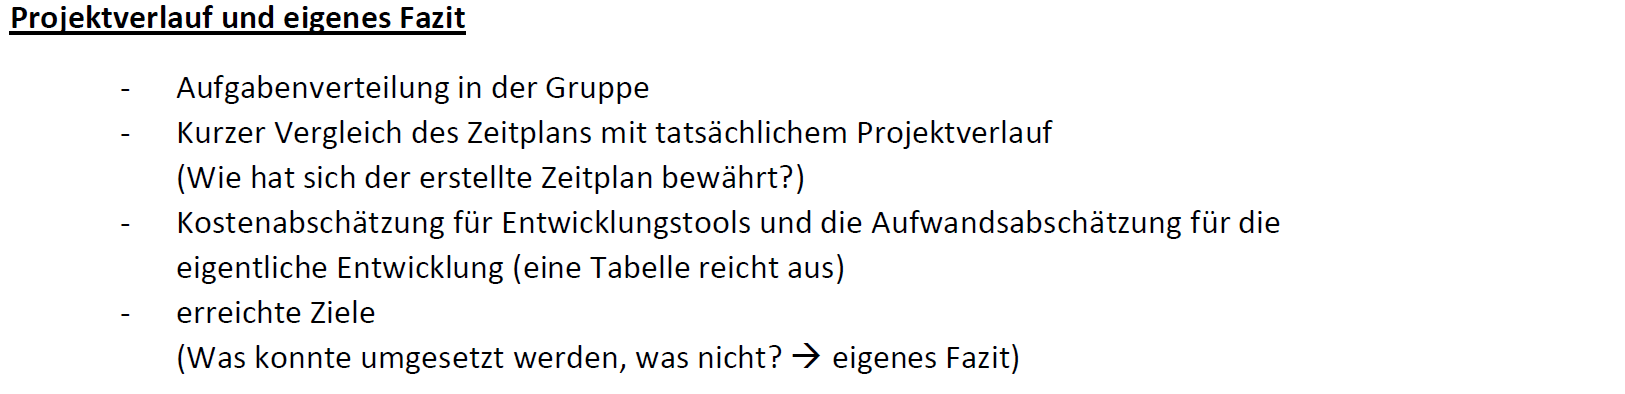
\includegraphics[scale=0.5]{images/projektverlauf.png}\\\\
\section{Fazit}
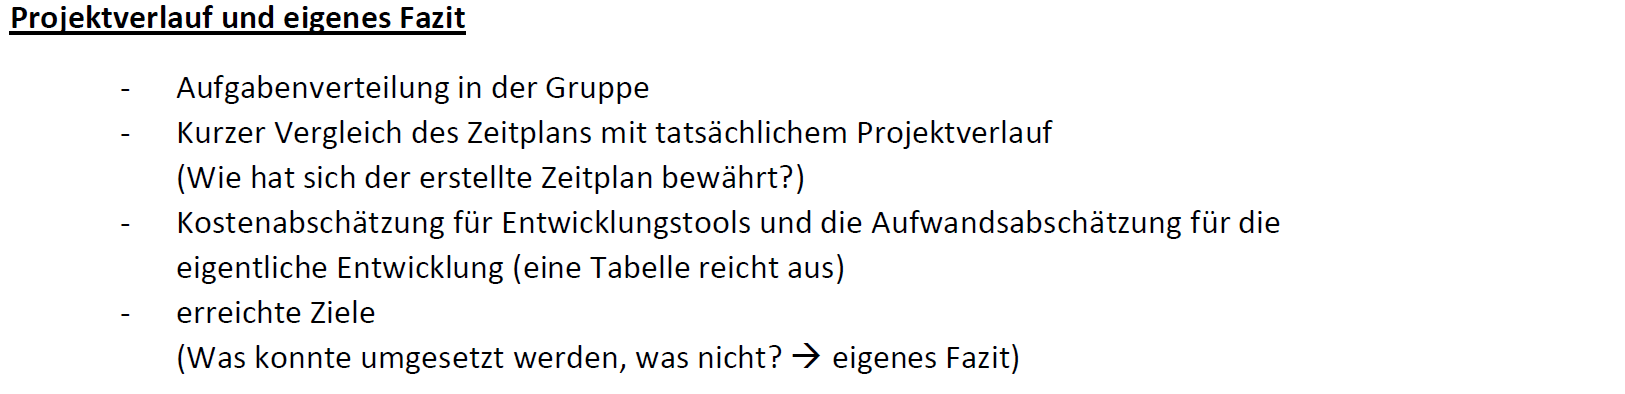
\includegraphics[scale=0.5]{images/projektverlauf.png}\\\\

\section{Statement von jedem Gruppenmitglied}

\includegraphics[scale=0.5]{images/statement.png}\\\\
\subsection{Hung Tran Duc}
\subsection{Elizaveta Ragosina}
\subsection{Philipp Plotz}
\subsection{Christoph Jurkowski}
\subsection{Niklas Fallik}
\subsection{Sheyda Hayatgheybi}

%----------------------------------------------------------------------------------------

\end{document}